% allgem. Dokumentenformat
\documentclass[12pt,landscape,oneside]{book}


% deutsche Silbentrennung
\usepackage[ngerman]{babel}

% Umlaute unter UTF8 nutzen

% Zeichenencoding
\usepackage[utf8]{inputenc}
\usepackage{lmodern}
\usepackage{fix-cm}

% mehrseitige Tabellen ermöglichen
\usepackage{longtable}

% Packet für Seitenrandabstände und Einstellung für Seitenränder
\usepackage[left=3cm, right=3cm, top=2.25cm, bottom=2.25cm]{geometry}

% neue Kopfzeilen mit fancypaket
\usepackage{fancyhdr} %Paket laden
\pagestyle{fancy} %eigener Seitenstil
\fancyhf{} %alle Kopf- und Fußzeilenfelder bereinigen
\fancyhead[L]{\nouppercase{\leftmark}} %Kopfzeile links
\fancyhead[C]{} %zentrierte Kopfzeile
\fancyhead[R]{\thepage} %Kopfzeile rechts
\renewcommand{\headrulewidth}{0.4pt} %obere Trennlinie
\setlength{\headheight}{15pt}

%Fußnoten
\usepackage{footnote}
\usepackage[perpage,symbol,stable]{footmisc}
\makeatletter
\newcommand\footnoteref[1]{\protected@xdef\@thefnmark{\ref{#1}}\@footnotemark}
\makeatother
\makesavenoteenv{tabular}
\makesavenoteenv{table}


% für Tabellen
\usepackage{array}
\usepackage{booktabs}
\usepackage{tabularx}
\newcolumntype{L}[1]{>{\raggedright\arraybackslash}p{#1}}

% Paket für Zeilenabstand
\usepackage{setspace}

% Verlinkungen innerhalb des Dokuments
\usepackage[hidelinks]{hyperref}
\hypersetup{allcolors=black,linktocpage,linktoc=all}
\newcommand{\recipe}[1]{%
    \hyperref[sec:#1]{\nameref{sec:#1} (S. \pageref{sec:#1})}
}

% Nummerirung der Rezepte abschalten
\setcounter{secnumdepth}{-2}

% Ungetestete Rezepte markieren
\usepackage[dvipsnames]{xcolor}
\newcommand{\unverified}[1][UNGEPRÜFTES REZEPT -- Anweisungen ggf. anpassen]{%
    \centering%
    \textcolor{yellow}{#1}%
    \flushleft%
}
\newcommand{\wip}[1][WORK IN PROGRESS]{%
    \centering%
    \textcolor{red}{#1}%
    \flushleft%
}

% weitere Pakete
% Grafiken aus PNG Dateien einbinden
\usepackage{graphicx}
\usepackage{tikzpagenodes}

% Titel- und Rückseite
\usepackage{pdfpages}

% Hintergrundbilder
\usepackage{transparent}
\usepackage{eso-pic}

% Einheiten
\usepackage{textcomp}
\newcommand{\cel}[1]{\textbf{#1\textdegree{}C}}
\newcommand{\mins}[1]{\textbf{#1 min}}
\newcommand{\std}[1]{\textbf{#1 Std.}}

% Schriftart
\renewcommand{\familydefault}{\sfdefault}
\date{}
\title{ }
\begin{document}
    
\includepdf[pages=-]{res/Munchies_front.pdf}
    \AddToShipoutPictureBG{\transparent{0.885}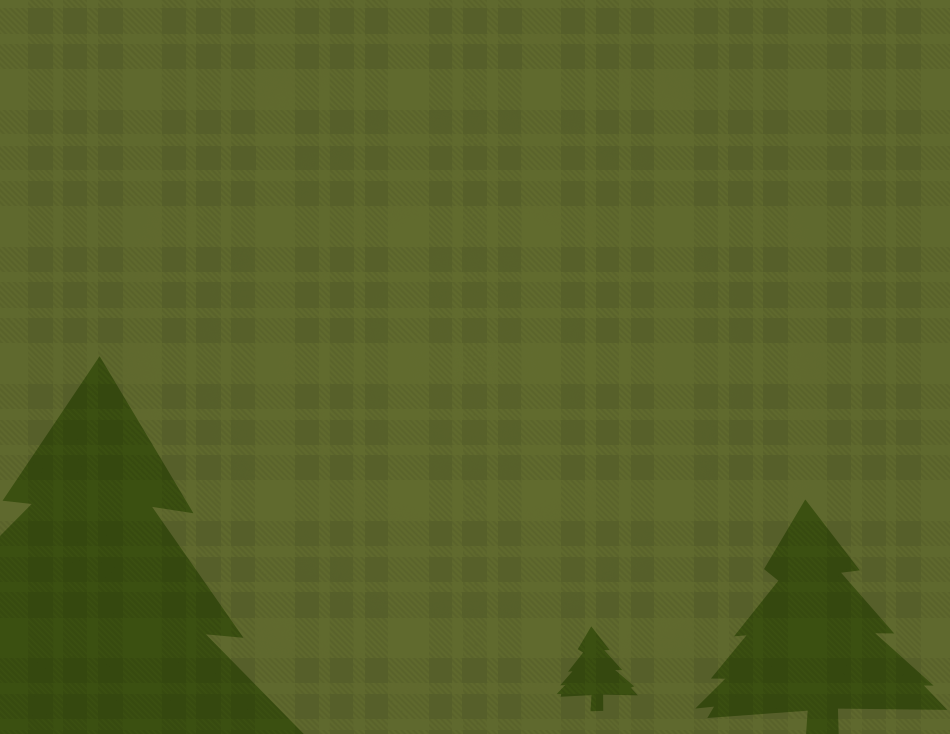
\includegraphics[width=\paperwidth,height=\paperheight]{res/Munchies_background.png}}

% Inhaltsverzeichnis anzeigen
%\newpage
    \pagenumbering{Roman}
    \setcounter{page}{1}
    \tableofcontents

    \fancyhead[L]{Inhaltsverzeichnis} %Kopfzeile links
%%%%

% Definiert Stegbreite bei zweispaltigem Layout
    \setlength{\columnsep}{25pt}

%%%%%%%%%%%% EINLEITUNG %%%%%%%%%%%%
%\twocolumn
    \newpage
    \pagenumbering{arabic}
    \fancyhead[L]{\nouppercase{\leftmark}} %Kopfzeile links

% 1,5 facher Zeilenabstand
    \onehalfspacing

% einzelne Kapitel


    \part{Deftiges}


    \chapter{Einzelnes}
    \section{Auberginenmus}
Ofen auf \cel{200} vorheizen.
\begin{longtable}{rlL{17.5cm}}
	1		&	Aubergine	&	längs halbieren, Gitterförmig einritzen und mit	\\
	2-3 EL	&	Olivenöl	&	beträufeln. Die Auberginenhälften für \std{ca. 1} backen, dann mit einem Löffel ausschaben (und falls nötig pürieren).	\\
	1 Zehe	&	Knoblauch	&	sehr fein schneiden und zum Mus geben.	\\
\end{longtable}

Würz-Vorschläge:
\begin{itemize}
	\item Ingwer, Chili, Zimt
	\item Rosmarin, Thymian, (Basilikum)
	\item Tahin, Tamarindenpaste, (Korianderkraut)
\end{itemize}
    \newpage
    \section{Bärbelbrot}
\begin{tikzpicture}[remember picture,overlay]
    \node[anchor=east,yshift=-4.5cm,inner sep=0pt] at (current page text area.east|-0,3cm) {\includegraphics[height=6cm]{res/Bärbelbrot.png}};
\end{tikzpicture}
\subsection*{Vorteig}\label{vorteig}
\begin{longtable}{rlL{15.9cm}}
	330ml				&	Wasser				&	auf \cel{40} erwärmen und mit	\\
	$1\frac{1}{2}$ EL	&	Anstellgut			&	und	\\
	330g				&	Roggenvollkornmehl	&	vermischen	\\
\end{longtable}

Den Vorteig abends zubereiten und \textbf{über Nacht} bei Zimmertemperatur (ca. \cel{20}) gehen lassen.\\
Dann $1\frac{1}{2}$ EL abnehmen und als Anstellgut in einem Schraubglas aufbewahren.

\subsection*{Hauptteig}
\begin{longtable}{rlL{16cm}}
	$\frac{3}{4}$ EL	&	Salz				&	in	\\
	330ml				&	Wasser				&	auflösen und auf \cel{40} erwärmen.	\\
	1 EL				&	Kümmel				&	mit	\\
	1 TL				&	Koriander			&	mörsern.	\\
	1 EL				&	Sesam				&	,	\\
	1 EL				&	Sonnenblumenkerne	&	und	\\
	1 EL				&	Leinsamen			&	mit Koriander-Kümmel Gemisch und	\\
	360g				&	Weizenvollkornmehl	&	vermischen und mit Salzwasser und	\\
						&	\nameref{vorteig}	&	zu einem Teig verkneten.	\\
\end{longtable}

Eine passende Kastenform einfetten und mit Sesam bestreuen, damit sich das Brot später besser herauslösen lässt.\\
Hauptteig in die Kastenform füllen und mit feuchten Fingern glattstreichen.
Dann Sesam andrücken und für \std{3 bis 6} gehen lassen.\\
Anschließend bei \cel{210} bis \cel{230} für \std{1} backen.
Danach sofort stürzen und abkühlen lassen.
    \newpage
    \section{Hot Things}\label{sec:hot_things}
Ofen auf \cel{180} vorheizen.
\begin{longtable}{rlL{16.75cm}}
    100g                &   Mehl            &   mit \\
    1TL                 &   Knoblauchpulver &   ,   \\
    1$\frac{1}{2}$TL    &   Paprikapulver   &   ,   \\
                        &   Salz \& Pfeffer &   ,   \\
    180ml               &   Sojamilch       &   und \\
    60ml                &   Wasser          &   mischen.    \\
    1                   &   Blumenkohl      &   in kleine Röschen schneiden und in die Panade tauchen, sodass sie vollständig bedeckt sind.
                                                Dann in \\
    100g                &   Panko\footnote{,,gewöhliche'' Semmelbrösel oder grob gemörserte Chips eignen sich ebenfalls.}
                                            &   wälzen und für \mins{25} backen.    \\
    240ml               &   BBQ-Sauce       &   mit \\
    1TL                 &   Sriracha Sauce  &   mischen und gebackene Röschen gleichmäßg damit bedecken und weitere \mins{20} backen.\\
\end{longtable}

Schmeckt gut mit \hyperref[sec:vegan_mayo]{veganer Mayonaise}
    \newpage
    \section{Caulicups}
\wip
\begin{longtable}{rlL{17.05cm}}
    4       &   große Kartoffeln    &   für \mins{ca. 30} kochen.   \\
    1       &   Zwiebel             &   hinzugeben und weitere \mins{10} kochen.
                                        Beides herausnehmen und \\
    200g    &   Blumenkohl          &   ins heiße Wasser geben und knapp \mins{10} kochen.
                                        Mit \\
            &   Salz \& Pfeffer     &   und \\
            &   Muskat              &   würzen und pürieren.    \\
\end{longtable}
Die abgekühlten Kartoffeln vorsichtig mit einem Löffel aushöhlen, von innen Salzen und mit Zwiebeln auskleiden.
Dazu werden die Schichten der Zwiebeln einzeln abgezogen und in die Kartoffeln gelegt.
Das Blumenkohlpüree hineingeben und bei \cel{200} für \mins{30-40} backen.

    \newpage
    \input{Rezepte/Chinakohl-Blitva}
    \newpage
    \section{Dashi}\label{sec:dashi}
\begin{longtable}{rlL{15.25cm}}
	$12,5$cm$^2$	&	Kombu					&	und	\\
	1				&	getrockneten Shiitake	&	in	\\
	180ml			&	Wasser					&	für mindestens \mins{30} einweichen lassen, dann mit wenig Hitze langsam zum Kochen bringen. \\
					&							&	Dann \textbf{nicht} kochen lassen, sondern sofort Kombu und Shiitake herausnehmen.
\end{longtable}

Kombu und Shiitake können für das nächste Dashi (wird etwas schwächer) im Gefrierfach aufgehoben werden.

Dashi wird z.B. für \recipe{ramen} oder \recipe{sushi_rice} verwendet.
    \newpage
    \section{Gazpacho}
\begin{tikzpicture}[remember picture,overlay]
    \node[anchor=east,yshift=-4.5cm,inner sep=0pt] at (current page text area.east|-0,3cm) {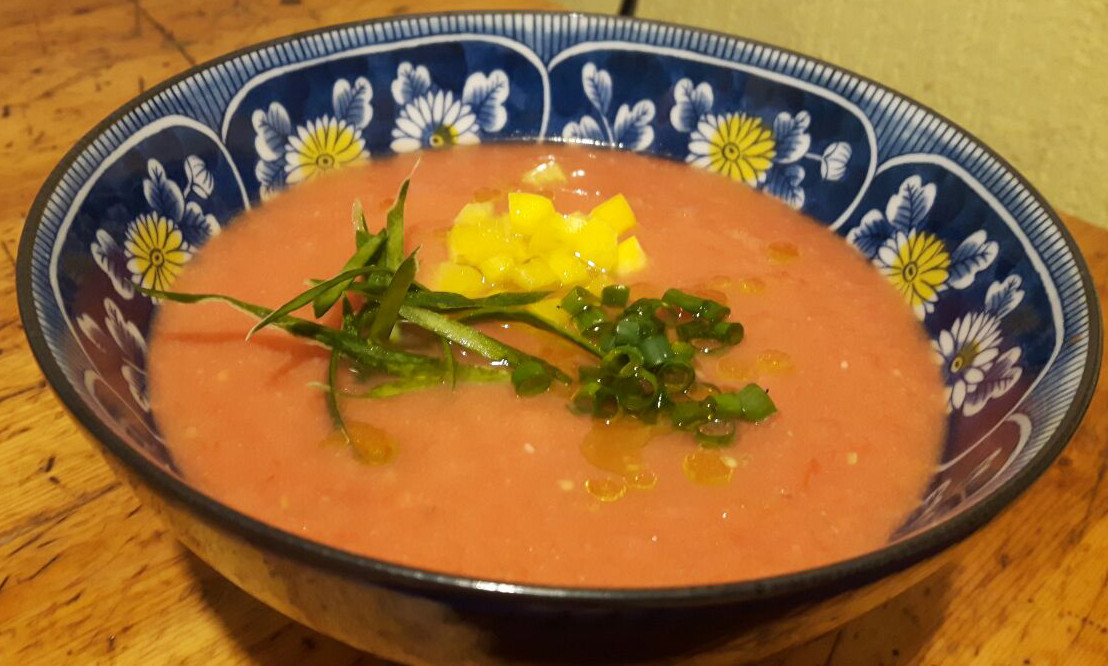
\includegraphics[height=4.5cm]{res/Gazpacho.jpg}};
\end{tikzpicture}
\begin{longtable}{rlL{16.46cm}}
    1       &   Gurke               &   schälen, entkernen und schneiden.
                                        Von\\
    1kg     &   Tomaten             &   die Stiele entfernen und schneiden.\\
    1       &   Paprika             &   entkernen, schneiden und einen Teil zum dekorieren\\
            &                       &   zur Seite legen.\\
    50g     &   Weißbrot            &   zerkleinern und alles zusammen mit\\
    2 EL    &   Essig               &   (Sherry oder Weißwein),\\
    3 EL    &   Olivenöl            &   und\\
    1 TL    &   Salz                &   pürieren.\\
    1 Zehe  &   Knoblauch           &   klein schneiden und dazugeben.\\
    2       &   Frühlingszwiebeln   &   schneiden und den weißen Teil dazugeben.
                                        Noch einmal kurz pürieren.\\
\end{longtable}
Das Weißbrot kann für eine dünnere Konsistenz weggelassen werden.
Ggf. kann man hierfür auch noch Eiswasser mitpürieren.
Man kann das Gazpacho auch mit Cumin verfeinern oder den Knoblauch weglassen, wenn man ein anderes Aroma möchte.
Gazpacho wird kalt serviert.
    \newpage
    \section{Gnocchi}
\begin{longtable}{rlL{18cm}}
	400g	&	Kartoffeln	&	(am besten alt und mehligkochend) in der Mikrowelle garen.
								Noch heiß stampfen und nach und nach	\\
	100g	&	Mehl		&	zugeben.	\\
\end{longtable}

Den Teig nachdem er abgekühlt ist zu etwa fingerdicken Schlangen rollen.
Die Schlangen in ca. 1,5 cm dicke Stücke schneiden und auf eine bemehlte Fläche legen.\\

Dann die Gnocchi mit einem Finger über eine Gabel rollen.
Dabei erzeugt die Gabel die charakteristischen Rillen und der Finger drückt eine Mulde in die Rückseite.\\

Wenn alle Gnocchi fertig sind, mit einem Tuch bedecken und Wasser salzen und kochen.
Die Gnocchi in das kochende Wasser gleiten lassen und mit einem Abseihlöffel herausnehmen, sobald sie an der Oberfläche schwimmen.
    \newpage
    \section{Sushi Reis}\label{sec:sushi_rice}
\subsection*{Sushi Su}\label{subsec:sushi_su}
\begin{longtable}{rlL{17.8cm}}
	75ml	&	Reisessig	&	mit\\
	37g		&	Zucker 		&	und\\
	19ml	&	Mirn/Sake	&	und\\
	1TL		&	Salz		&	mischen, bis sich Zucker und Salz vollständig gelöst haben.\\
\end{longtable}

\subsection*{Reis}
\begin{longtable}{rlL{17cm}}
	300g	&	Sushi Reis			&	waschen (3-4 mal, oder bis das Wasser klar ist) und zusammen mit\\
	360ml	&	\recipe{dashi}	&	in einen Topf geben und \mins{20-30} ziehen lassen.\\
			&			 			&	Dann köcheln lassen, bis alles Wasser weg ist und \mins{15} stehen lassen.\\
			&	\nameref{subsec:sushi_su}	&	vorsichtig mit einem Holzlöffel einrühren und währenddessen Luft zufächern.\\
			&						&	Mit einem feuchten Tuch bedecken und auf (etwas über) Zimmertemperatur abkühlen lassen.\\
\end{longtable}
    \newpage
    \section{Tomaten--Apfel--Aufstrich}
\begin{longtable}{rlL{14.67cm}}
    1       &   Apfel           &   reiben, \\
    1       &   Zwiebel         &   und \\
    1 Zehe  &   Knoblauch       &   fein schneiden, und alles mit \\
    150g    &   Tomatenmark     &   und \\
            &   Salz \& Pfeffer &   vermengen (nicht zu gründlich).\\
\end{longtable}

    \newpage
    \section{Vegane Mayonaise}\label{sec:vegan_mayo}
\begin{longtable}{rlL{16cm}}
    50ml            &   Sojamilch       &   mit \\
    1TL             &   Zitronensaft    &   ,   \\
    1TL             &   Senf            &   und \\
                    &   Salz \& Pfeffer &   in ein geeignetes Gefäß geben und nach und nach \\
    bis zu 100ml    &   Öl              &   hineinpürieren, bis die Masse die richtige Konsistenz hat.  \\
\end{longtable}

Lässt sich natürlich auch mit weiteren Gewürzen (z.B. Knoblauch für Aioli) verfeinern.
Passt z.B. zu \nameref{sec:hot_things}
    \newpage
%\section{}
\begin{longtable}{rlL{25cm}}
\end{longtable}
%\newpage


    \chapter{Gerichte}
%\section{Vorspeise (working title)}
	
	\begin{itemize}
		\item Apfelscheiben (Häppchengröße!)
		\item Tomatenbällchen (vgl. La Technique S. tba)
		\item Balsamicocreme
		\item Basilikum
	\end{itemize}
	
\section{Apfelblüten auf Gorgonzolasoße (work in progress)}

	\subsection*{Apfelblüten}
		
		\begin{itemize}
			\item Nudelteig:
				\begin{itemize}
					\item 300g Mehl
					\item 150ml Wasser
					\item 1/2TL Salz
					\item 2TL Olivenöl
				\end{itemize}
			\item Apfelstückchen eindrehen
		\end{itemize}
		
		\begin{tabular}{rlL{10cm}}
			
		\end{tabular}\\
			
	\subsection*{Gorgonzolasoße}
		\begin{tabular}{rlL{9cm}}
			
		\end{tabular}\\
	
\section{Nachspeise (working title)}
	\begin{itemize}
		\item Mürbteigplätzen(Häppchengröße!):
			\begin{itemize}
				\item 3 Teile Mehl
				\item 2 Teile Margarine
				\item 1 Teil Zucker
				\item ein paar Mandeln
			\end{itemize}
		\item Schlagsahne
		\item eingelegte Pflaumen  %TODO
		\item Basilikumblatt
	\end{itemize}
%\newpage
    \section{Bumblebeets mit Brokkolieis}
\begin{tikzpicture}[remember picture,overlay]
    \node[anchor=east,yshift=-4cm,inner sep=0pt] at (current page text area.east|-0,3cm) {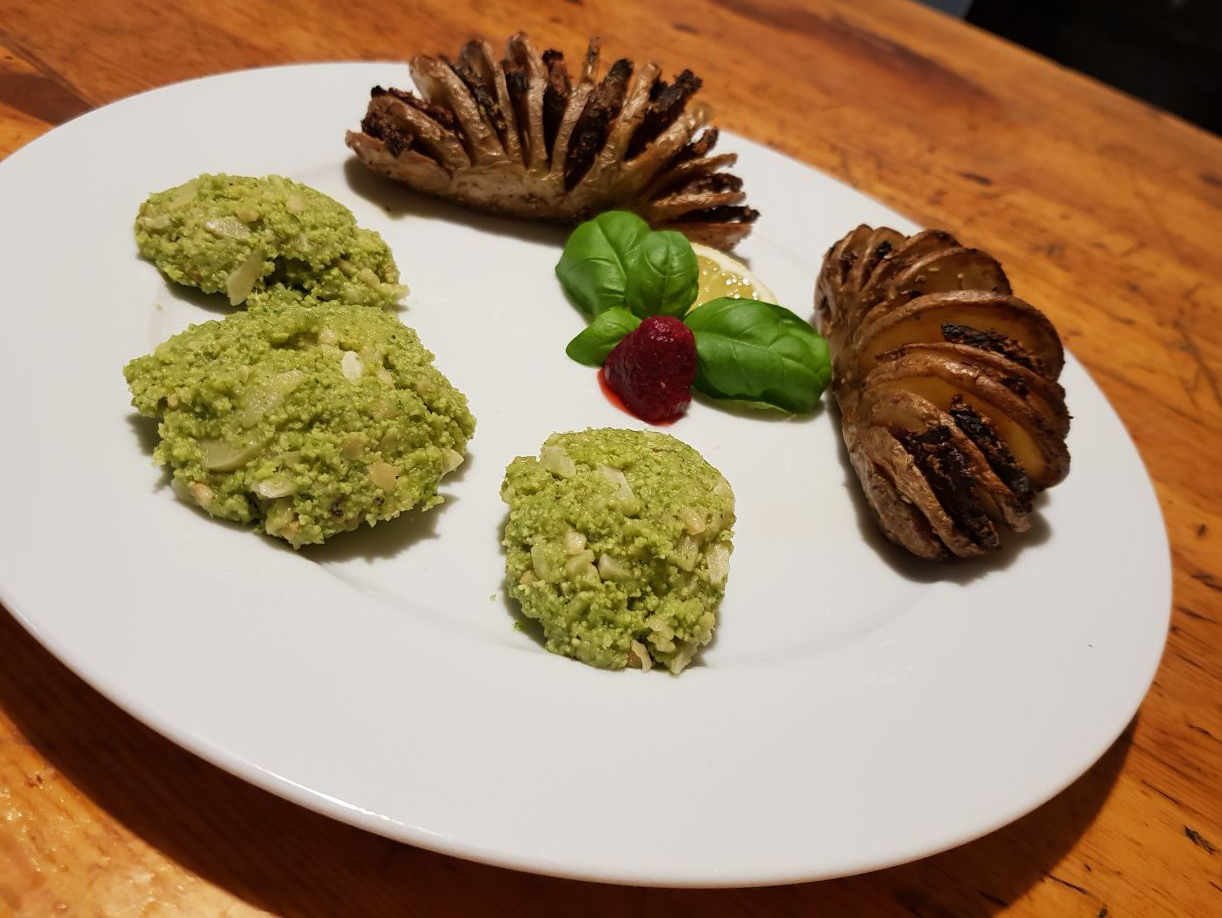
\includegraphics[height=5cm]{/Users/dertoast/Documents/Zeug/Küche/Munchies/res/bumblebeets.png}};
\end{tikzpicture}
\subsection*{Brokkoli-Eiscreme}\label{subsec:broc-icecream}
\subsubsection*{Eismasse}
\begin{longtable}{rlL{15,8cm}}
    200g                    &   Brokkoli        &   kurz in    \\
    100g                    &   Butter\footnote{gerne auch vegan z.B. \href{https://www.bio123.de/produkt/naturli/naturli-organic-vegan-block-200g}{Naturli vegan block}
									        oder \href{https://www.alsan.de/alsan-bio/}{Alsan}}
                                                &   dünsten.
                                                    Dann mit    \\
    100ml                   &   Haselnussmilch  &   ablöschen und   \\
    $\frac{1}{2}$TL (4g)    &   Salz            &   sowie \\
    20ml                    &   Weißwein        &   zugeben und pürieren    \\
\end{longtable}
\subsubsection*{Frieren}
\emph{Die Frierzeiten sind abhängig von Menge und Gefrierfach/-schrank.}
\begin{longtable}{rlL{14,6cm}}
    Ca. $\frac{3}{4}$ Std.  &   im Gefrierfach                  &   anfrieren lassen.   \\
    Ca. 1 Std.              &   weiter frieren                  &   , dabei aber \mins{alle 20} mit einem Schneebesen verquirlen \\
    \textbf{50g}            &   \textbf{Mandelstifte}           &   und \\
    \textbf{50g}            &   \textbf{gehackte Haselnüsse}    &   unterrühren und dann weitere    \\
    1 Std.                  &   frieren                         &   und dabei \mins{alle 20} mit einem Teigschaber umrühren. \\
\end{longtable}

\subsection*{Kartoffel-Rote Beete-Fächer}\label{subsec:bumblebeets}
Die Gewürz-Öl Mischungen sollten zuerst zubereitet werden, damit die Aromen besser durchziehen können.
\subsubsection*{Rote Beete}\label{subsubsec:beets}
\begin{longtable}{rlL{16.9cm}}
    1 TL            &   Kreuzkümmel &   zusammen mit    \\
    2 TL            &   Senfkörnern &   mörsern. Von    \\
    $\frac{1}{2}$   &   Zitrone     &   Zesten reißen und fein hacken.  \\
    3 EL            &   Olivenöl    &   und gemöserte Gewürze damit zu einer Würzpaste vermischen.  \\
    2               &   rote Beeten &   in 3mm dicke Scheiben schneiden und mit Würpaste bestreichen.\\
\end{longtable}

\subsubsection*{Kartoffeln}
Ofen auf \cel{200} vorheizen
\begin{longtable}{rlL{16.8cm}}
    3       &   Knoblauchzehen      &   und \\
            &   Rosmarin            &   möglichst fein schneiden und mit    \\
    7 EL    &   Olivenöl            &   zu einem Würzöl vermischen. \\
    4       &   große Kartoffeln    &   scheibenartig (ca. 7mm) einschneiden (nicht ganz durch, sie sollen später aufgefächert werden). \\
\end{longtable}
Die Kartoffeln mit Würzöl bestreichen und für \mins{20} vorbacken, bis man sie auffächern kann, ohne sie dabei zu zerbrechen.
Dann die gewürzten \nameref{subsubsec:beets}-Scheiben in die Lücken stecken und weitere \mins{20-30} backen.

Die fertigen \nameref{subsec:bumblebeets} mit je einer Kugel \nameref{subsec:broc-icecream} und einem Schnitz Zitrone servieren.
Zur Dekoration eignen sich Basilikumblätter und Himbeeren, da beides geschmacklich auch sehr gut passt.

    \newpage
    \section{Gigantes Plaki auf Auberginen}
\begin{longtable}{r l L{16.4cm} }
	1				&	große Zwiebel	&	würfeln und zusammen mit	\\
	2				&	Karotten		&	und	\\
	$\frac{1}{8}$	&	Sellerie		&	in \\
					&	Olivenöl		&	anschwitzen. Mit	\\
	2-3 Dosen		&	Tomaten			&	ablöschen und mindestens 1 Stunde köcheln lassen.	Mit\\
	1 Bund			&	Dill			&	, \\
	1 Bund			&	Petersilie		&	, Salz und Pfeffer abschmecken. \\
					&					&	Den Ofen auf \cel{180} vorheizen. \\
	1				&	Aubergine		&	in ca. 1cm dicke Scheiben schneiden und Bitterstoffe entziehen\footnote{Dazu werden die Auberginen mit Salz bestreut und sobald keine Salzkörner mehr zu sehen sind, die entzogene Flüssigkeit mit einem Küchentuch abgetupft.}.
											Die Auberginenscheiben umdrehen und von der anderen Seite wiederholen. Mit\\
					&	Olivenöl		&	beträufeln und in einer möglichst breiten Auflaufform \mins{15-20} backen.
											Nach der Hälfte der Zeit wenden.	\\
	500g			&	Riesenbohnen	&	abgießen, mit klarem Wasser abbrausen und unter die Tomatensoße mischen.
														Dann auf die Auberginen geben und für ca. \mins{90} bei \cel{150} backen.	\\
\end{longtable}
    \newpage
    \section{Ramen}\label{sec:ramen}
\subsection*{Suppenbasis}\label{subsec:ramen_soup}
\begin{longtable}{rlL{16.2cm}}
	2 Zehen	&	Knoblauch			&	und	\\
	1,5cm	&	Ingwer				&	fein schneiden.	\\
	1		&	Frühlingszwiebel	&	in Ringe schneiden und dabei den weißen vom grünen Teil trennen.	\\
	2 EL	&	Sesamöl				&	in einem Topf erhitzen und	Knoblauch, Ingwer und den weißen Teil der Frühlingszwiebeln bei schwacher bis mittlerer Hitze anschwitzen.	\\
	2 EL	&	Doubanjiang\footnote{fermentierte Bohnenpaste (mit oder ohne Chili)}	&	und \\
	2 EL	&	Miso				&	(weiß oder rot je nach Geschmack) zugeben und konstant rühren, sodass sie nicht anbrennen.	\\
	1 EL	&	Sake				&	hinzugeben. (Das hilft dabei, festgebackene Stückchen zu lösen.)	\\
	1 EL	&	weißer Sesam		&	mörsern und zusammen mit	\\
	2 EL	&	heller Sojasoße		&	hinzugeben.	\\
	240ml	&	Sojamilch			&	nach und nach (!) hinzugeben.
										Dann	\\
	120ml	&	\recipe{dashi}		&	hinzufügen und mit	\\
			&	weißem Pfeffer		&	und	\\
			&	Salz				&	abschmecken.	\\
\end{longtable}
Die Suppenbasis darf \textbf{nicht} kochen, sonst fällt das Miso aus!
Anschließend die Basis nach belieben mit Wasser aufgießen.
Für ein besonders indviduelles Geschmackserlebnis kann man das auch direkt in der Schüssel machen.
\subsection*{Nudeln}\label{subsec:ramen_noodles}
\begin{longtable}{rlL{16.7cm}}
	250g	&	Mehl (Typ 405)	&	mit \\
	15g		&	Gluten			&	vermischen und eine Mulde hineindrücken. \\
	3g		&	Salz			&	und \\
	2g		&	Na$_2$CO$_3$	&	in \\
	100ml	&	warmen Wasser	&	auflösen und in die Mulde geben.
									Von innen nach außen einrühren, sodass das Mehl nach und nach aufgenommen wird. \\
\end{longtable}

Sobald der Teig nicht mehr klebrig ist, das restliche Mehl nach und nach in den Teig einfalten bis ein glatter Teig entsteht.
Den Teig für ca \mins{30} im Kühlschrank ruhen lassen.

In einer Nudelmaschine ausrollen und dabei bei Bedarf wieder falten, bis der Teig dünn genug ist, um zu Nudeln mit quadratischem Querschnitt zu schneiden.

Ungesalzenes Wasser kochen und die Nudeln für \textbf{30 Sekunden} kochen.
\subsection*{Toppings}\label{subsec:ramen_toppings}
Offensichtlich nach belieben (das ist ja gerade das schöne an Ramen).
Aber geeignet sind (unter anderem!):
\begin{itemize}
	\item der (schon geschnittene) grüne Teil der Frühlingszwiebel
	\item (Ramen-)Eier (Rezept t.b.a.)
	\item (am besten frische) Bohnensprösslinge (Soja oder Mungo)
	\item Mais
	\item Kimchi
	\item Röstzwiebeln (ganz zum Schluss oben drauf, weichen sofort durch)
\end{itemize}
\subsection*{Servieren}
\nameref{subsec:ramen_noodles} zubereiten, dann sofort mit \nameref{subsec:ramen_soup} auffüllen und mit \nameref{subsec:ramen_toppings} garnieren.
Schlürfen nicht vergessen!
    \newpage
    \section{Spanakoriso}
\begin{longtable}{rlL{16.1cm}}
	3		&	Frühlingszwiebeln	&	in \\
			&	Olivenöl			&	anschwitzen und \\
	600g	&	Spinat				&	dazugeben (bei frischem Spinat: dünsten, bis er zusammenfällt), dann \\
	1 Dose	&	Stückige Tomaten	&	und \\
	400ml	&	Wasser				&	dazugeben und mit Salz, Pfeffer und \\
	1 Hand	&	Dill				&	abschmecken.\\
	150g	&	Reis				&	einrühren und unter Rühren köcheln lassen, bis das Wasser vollständig aufgesaugt ist
										(wenn der Reis noch hart ist, weiteres Wasser hinzufügen.
\end{longtable}
    \newpage
    \section{Stapfelrisotto}
\begin{longtable}{rlL{17,06cm}}
    3       &   Zwiebeln        &   fein und \\
    100g    &   Steinpilze      &   grob schneiden und in  \\
    etwas   &   Butter\footnote{gerne auch vegan z.B. \href{https://www.bio123.de/produkt/naturli/naturli-organic-vegan-block-200g}{Naturli vegan block}
                            oder \href{https://www.alsan.de/alsan-bio/}{Alsan}}
                                &   anschmoren.  \\
    2       &   Äpfel           &   in Stücke schneiden und mit \\
    200g    &   Risottoreis     &   zusammen in die Pfanne geben.
                                    Etwas braten lassen, dann mit   \\
    150ml   &   Weißwein        &   ablöschen und kochen lassen.
                                    Dabei unter ständigem Rühren nach und nach  \\
    500ml   &   Gemüsebrühe     &   zugeben.    \\
    75g     &   Parmesan        &   reiben und unterrühren, wenn die Flüssigkeit fast vollständig verkocht und aufgesaugt wurde.
                                    Mit \\
            &   Salz \& Pfeffer &   abschmecken.\\
\end{longtable}

Das Gericht lässt sich gut verfeinern, indem man z.B. \textbf{Walnüsse} röstet und über das fertige Risotto streut.\\
Als Ersatz für die Steinpilze (die ja nicht immer leicht zu finden und im Laden meistens teuer sind) eignen sich Pfifferlinge.
Champignons sind auch möglich, verlieren beim Garen allerdings deutlich mehr Flüssigkeit und sollten daher erst mit dem Reis in die Pfanne gegeben werden.
Da sie weniger Geschmacksintensiv sind, empfiehlt es sich auch etwas mehr zu verwenden.
    \newpage
    \section{Gefüllte Mangoldblätter mit Mango:ldchutney in Spinatschüsseln}
\begin{tikzpicture}[remember picture,overlay]
    \node[anchor=east,yshift=-4.5cm,inner sep=0pt] at (current page text area.east|-0,3cm) {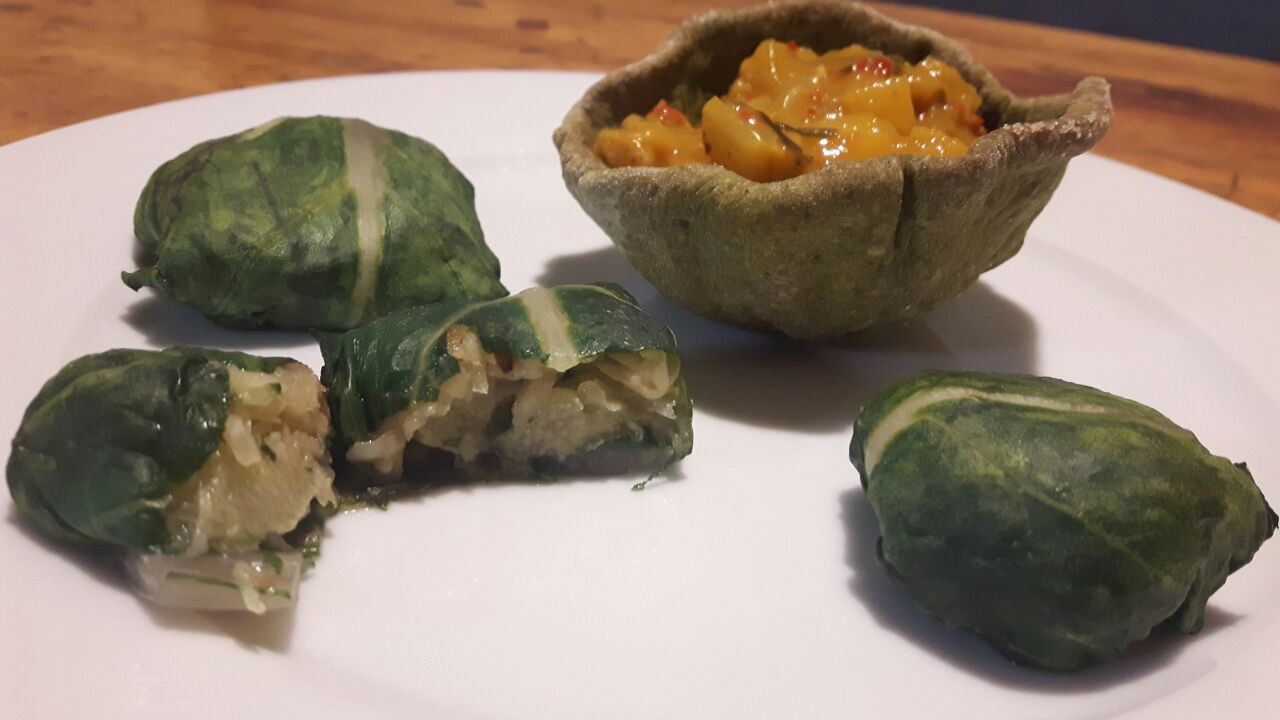
\includegraphics[height=4cm]{res/mango*ld.jpeg}};
\end{tikzpicture}
\subsection*{Spinaschüsseln}\label{subsec:spinach-bowls}
\begin{longtable}{rlL{17.1cm}}
    50g     &   Spinat          &   mit etwas   \\
            &   Wasser          &   pürieren und    \\
    1 EL    &   Sauerteigansatz &   dazugeben.  \\
            &   Weizenmehl      &   einkneten, bis der Teig pizzaartige Konsistenz hat.
                                    Über Nacht gehen lassen   \\
    1 TL    &   Salz            &   unterkneten.    \\
\end{longtable}
Ofen auf \cel{200} vorheizen.
Einen Apfel (oder etwas anderes Rundes von etwa gleicher Größe) zur Hälfte in Alufolie einwickeln, um kleine (gleichmäßige) Schüsseln daraus zu formen.
Den Teig zu kleinen Kugeln formen, plattdrücken und mit \textbf{ganzen Spinatblättern} belegen.
Fertig ausrollen und auf die mit Aluschüsseln legen und so für \mins{10} backen.
Die Aluschüsseln herausnehmen und die Teigschüsseln mit der Öffnung nach oben für weitere \mins{5--10} backen.

\subsection*{Mango*ldchutney}\label{subsec:chutney}
\begin{longtable}{rlL{16.2cm}}
    1               &   Mangold         &   putzen und die Blätter vom Stiel trennen.
                                            Die Stiele klein würfeln (ca. 2cm$^2$) zusammen mit \\
    1               &   Zwiebel         &   und \\
    1cm             &   Ingwer          &   für \mins{ca. 10} in  \\
    1--2 EL         &   Butter\footnote{gerne auch vegan z.B. \href{https://www.bio123.de/produkt/naturli/naturli-organic-vegan-block-200g}{Naturli vegan block}
									        oder \href{https://www.alsan.de/alsan-bio/}{Alsan}}
                                        &   anschwitzen.    \\
    1               &   Chili           &   in \\
    1 TL            &   Tomatenmark\footnote{Das Tomatenmark hilft dabei, die Chili besser schneiden zu können, ohne dass die Kerne wegspringen.}
                                        &   zu einem feinen Muß schneiden und hinzugeben.   \\
    $\frac{1}{2}$   &   Mango           &   Würfeln und dazugeben.  \\
    1 TL            &   Zitronensaft    &   und \\
    2--3 EL         &   Apfel-Mango-Saft\footnote{oder ein anderer passender Saft}
                                        &   hinzugeben und weitere \mins{10} köcheln lassen.
                                            Salzen und Pfeffern.    \\
\end{longtable}

\subsection*{gefüllte Mangoldblätter}\label{subsec:filled_chard}
\begin{longtable}{rlL{14.45cm}}
    Die                         &   Mangoldblätter      &   \mins{1} blanchieren.   \\
    200g ($\frac{1}{2}$ Knolle) &   Sellerie            &   schälen und reiben.
                                                            Dann zusammen mit   \\
    1                           &   Zwiebel             &   dünsten bis der Sellerie weich ist. \\
    1--2 Stangen                &   Rhabarber           &   schälen und in 1--2cm lange Stücke schneiden.
                                                            \mins{1--2} blanchieren. \\
    je 1                        &   Mangoldblatt        &   mit Selleriemasse ,,bestreichen'',  \\
    je $\frac{1}{2}$ TL         &   Dill                &   darauf verteilen, salzen und pfeffern,   \\
    je 1--2                     &   Rhabarberstückchen  &   darauf legen und mit    \\
    je 1 Prise                  &   Zimt                &   bestreuen.
                                                            Zufalten, sodass kleine Päckchen entstehen und für \mins{ca. 5} backen.  \\
\end{longtable}
Etwas \nameref{subsec:chutney} in die \nameref{subsec:spinach-bowls} geben und zusammen mit den \hyperref[subsec:filled_chard]{gefüllten Mangoldblättern} auf den Teller legen.
    \newpage


    \part{Süßes}


    \chapter{Kuchiges}
    \section{Apfelkuchen Othello}
\begin{longtable}{rlL{16.9cm}}
	135g	&	Butter\footnote{gerne auch vegan z.B. \href{https://www.bio123.de/produkt/naturli/naturli-organic-vegan-block-200g}{Naturli vegan block}
									oder \href{https://www.alsan.de/alsan-bio/}{Alsan}}
								&	schmelzen und etwas abkühlen lassen.
									Währenddessen	\\
	240g	&	Mehl			&	mit	\\
	130g	&	Zucker			&	,	\\
	1 Pck.	&	Vanillezucker	&	,	\\
	1 Prise	&	Salz			&	,	\\
	1 TL	&	Backpulver		&	und	\\
	1 TL	&	Natron			&	vermischen.	\\
	100g	&	Kuvertüre		&	grob hacken,	\\
	ca. 50g	&	Kaffeebohnen	&	grob mörsern und zusammen mit	\\
	250g	&	Apfelmus		&	und der (gerade noch) flüssigen Butter so lange unterrühren, bis ein glatter Teig entsteht (nicht länger, sonst wird der Teig zu fest).	\\
	1-2		&	Äpfel			&	schneiden und zur Dekoration auf dem Teig verteilen.\\
\end{longtable}

Den Teig in einer (eingefetteten) 25cm-Springform für ca. \mins{35} bei ca. \cel{190} backen.
    \newpage
    \section{Brownies}
Ofen auf \cel{180} vorheizen.\\

\begin{longtable}{rlL{17.3cm}}
	550g	&	Schokolade		&	in zwei Hälften teilen und eine Hälfte schmelzen, die andere Hälfte grob hacken und beiseite legen. \\
	275g	&	Butter			&	schmelzen und mit \\
	300g	&	Zucker			&	und \\
	100ml	&	Buttermilch		&	glatt rühren. \\
	5		&	Eier			&	mit \\
	4-5TL	&	Vanillepaste	&	hineinschlagen.\\
			&					&	Dann die geschmolzene Schokolade einrühren. \\
	150g	&	Mehl			&	mit \\
	100g	&	Kakao			&	und \\
	2EL		&	Salz			&	vermischen und unterheben. (Nicht zu glatt rühren, sonst werden sie nicht fudgy!)\\
			&					&	Zum Schluss die gehackte Schokolade unterheben. \\
\end{longtable}

Die gesamte Masse in ein 25cm$\times$40cm Backblech geben und bei \cel{175} für \mins{20} backen oder mit einem Topping nach Wahl versehen und entsprechende Backtemperatur und -dauer beachten.
    \subsection*{Toppings}
    \subsubsection{Cheesecake-Topping}
\begin{longtable}{rlL{15.7cm}}
	550g	&	Frischkäse 				& mit \\
	370g	&	Griechischem Joghurt	& , \\
	4		&	Eiern 					& , \\
	2 Pck	&	Vanillezucker 			& , \\
	3 EL	&	Speisestärke 			& , \\
	115g	&	Zucker 					& und \\
 	400 g	&	Himbeeren 				& verrühren und Luft entweichen lassen. \\
\end{longtable}

Auf den (ungebackenen) Brownie-Teig geben und zusammen bei \cel{175} für \mins{25-30} backen.
    \subsubsection{Walnuss-Karamell-Topping}
Brownies fertig backen, dann:\\

\begin{longtable}{rlL{17.9cm}}
	200g	&	Zucker		&	vorsichtig schmelzen (bis leichte Bräunung eintritt) \\
	90g		&	Butter		&	in Stücke teilen und hinzugeben. (Vorsicht, Spritzgefahr!)
								Verrühren, bis die Butter vollständig geschmolzen ist. \\
	120ml	&	Sahne		&	unter Rühren hinzugeben (Vorsicht, noch mehr Spritzgefahr!)
								Ca. \mins{1} köcheln lassen. Vom Herd nehmen und \\
	200g	&	Walnüsse	&	hacken, anrösten und zusammen mit \\
	1TL		&	Salz		&	unterrühren. \\
\end{longtable}

Das fertige Topping auf den Brownies verteilen.
%\newpage
%\section{Oreo-Spekulatius-Käsekuchen mit Teespiegel}
\unverified
\subsection*{Der Oreoboden}
\begin{longtable}{rlL{17.7cm}}
	100ml	&	Espresso	&	mit \\
	50g		&	Zucker		&	zu dickflüssigem Sirup kochen.\\
	200g	&	Oreos		&	in Cremefüllung und Kekse teilen. \\
	100g	&	Butter		&	schmelzen und mit zerbröselten Keksen mischen. Gut die Häfte davon am Boden der Springform platt drücken. \\
			&				&	Die Cremefüllung mit  \\
	2 EL	&	Frischkäse	&	und Kaffeesirup glatt rühren und darauf verteilen. Alles mit restlicher Bröselmasse abdecken und ca. \mins{30} kaltstellen. \\
\end{longtable}

Ein Blech mit Wasser\footnote{Die erhöhte Luftfeutigkeit im Ofen macht den Kuchen deutlich saftiger.\label{humidity}} füllen und zum Vorheizen in den Ofen stellen (\cel{160}). \\

\subsection*{Die Spekulatiuscreme}
\begin{longtable}{rlL{16.5cm}}
	75g		&	Speisestärke		&	mit \\
	150g	&	Zucker				&	, \\
	1 Pck	&	Vanillezucker		&	, \\
	200g	&	Spekulatiuscreme	&	und \\
	1kg		&	Quark				&	verquirlen. \\
	200g	&	Schlagsahne			&	und \\
	2		&	Eier (M)			&	vorsichtig unterrühren. \\
\end{longtable}

Die Masse auf den Boden in der Springform füllen. Nach \std{1-2} Wartezeit\footnote{Die Luft muss vollständig aus dem Teig entweichen, damit er nicht zusammenfällt.\label{wait}} glatt ruckeln und ca \mins{10} backen. Ofen auf \cel{125} runterdrehen und \mins{85} backen. Den Kuchen langsam abkühlen lassen und für die Glasur kurz ins Gefrierfach stellen. \\

\subsection*{Der Teespiegel}
\begin{longtable}{rlL{15.4cm}}
	10g			&	Gelatine			& in  \\
	60ml		&	kaltem Wasser		&  auflösen. \\
	1 kl Tasse	&	starken Früchtetee	& kochen und mit \\
	150g		&	Glucosesirup\footnote{Verhindert das Kristallisieren des Zuckers und macht die Glasur dadurch klarer.} & und \\
	150g		&	Zucker				& auf ca 75ml reduzieren. \\
	100g		&	süße Kondensmilch	& und gelöste Gelatine hinzufügen. \\
	150g		&	weiße Schokolade	& darin auflösen und pürieren.  Wenn die Masse auf ca. \cel{35} abgekühlt ist,  über den kalten Kuchen gießen.\\
\end{longtable}
    \newpage
    \section{Orangen-Käsekuchen}
\subsection*{Der Boden}
\begin{longtable}{rlL{18.6cm}}
	200g	&	Kekse	&	(Butter-Mandelblätter oder Karamellgebäck) fein zerbröseln. \\
	100g	&	Butter	&	schmelzen und mit zerbröselten Keksen mischen und am Boden der Springform platt drücken. \\
\end{longtable}

 Ein Blech mit Wasser füllen und zum Vorheizen (auf \cel{160}) in den Ofen stellen. \\

\subsection*{Die Quarkcreme}
\begin{longtable}{rlL{17.2cm}}
	150g	&	Zucker			&	mit \\
	1 Pck	&	Vanillezucker	&	, \\
	1kg		&	Quark			&	und Zesten von \\
	3		&	Orangen			&	verquirlen.
									Den Saft von zweien mit \\
	75g		&	Speisestärke	&	anrühren und mit verrühren\\
	200g	&	Schlagsahne		&	und \\
	2		&	Eier (M)		&	vorsichtig unterrühren.
									Die Masse auf den Boden in der Springform füllen.\\
\end{longtable}

Nach \std{1-2} Wartezeit glatt ruckeln und ca \mins{10} backen. Ofen auf \cel{125} runterdrehen und \mins{85} backen.
Den Kuchen langsam abkühlen lassen. \\
Zum Schluss die dritte Orange filetieren und zum Dekorieren benutzen.
    \newpage
    \section{Rhababercrumble in Bananen-Schale}
Ofen auf \cel{180} vorheizen.
\subsection*{Bananen-Mürbeteig}\label{subsec:banana_shortcrust}
\begin{longtable}{rlL{18.54cm}}
    250g            &   Mehl    &   mit \\
    75g             &   Zucker  &   ,   \\
    $\frac{1}{2}$   &   Banane  &   und \\
    125g            &   Butter\footnote{\label{foot:butter}gerne auch vegan z.B. \href{https://www.bio123.de/produkt/naturli/naturli-organic-vegan-block-200g}{Naturli vegan block}
                                    oder \href{https://www.alsan.de/alsan-bio/}{Alsan}}
                                &   mischen\footnote{Mürbeteig sollte immer möglichst kalt verarbeitet werden und darf nicht zu gleichmäßig verknetet werden.} und kaltstellen. \\
\end{longtable}

\subsection*{Crumble}\label{subsec:crumble}
\begin{longtable}{rlL{16.68cm}}
    250g    &   Mehl            &   mit \\
    80g     &   braunem Zucker  &   und \\
    1 Prise &   Salz            &   mischen. \\
    170g    &   Butter\footnoteref{foot:butter}
                                &   würfeln und reinkneten\footnote{Nicht zu viel kneten, die größeren Krümel sind immer am leckersten}, bis eine krümelige Masse entsteht und kaltstellen.  \\
\end{longtable}

\subsection*{Füllung}\label{subsec:rhubarb-filling}
\begin{longtable}{rlL{17.23cm}}
    800g    &   Rhabarber       &   schälen und in 3cm-Stücke schneiden.    \\
    1TL     &   Vanillepaste    &   ,   \\
    150g    &   brauner Zucker  &   und \\
    5TL     &   (Mais-)Mehl     &   unterrühren.    \\
\end{longtable}

\subsection*{Finish}
\begin{longtable}{rlL{16.85cm}}
                    &   \nameref{subsec:banana_shortcrust}  &   in eine Springform drücken. (mit Rand!) \\
    4$\frac{1}{2}$  &   Bananen                             &   pürieren und auf dem \nameref{subsec:banana_shortcrust} verstreichen.    \\
                    &   \nameref{subsec:rhubarb-filling}    &   einfüllen und das ganze mit \\
                    &   \nameref{subsec:crumble}            &   abdecken und für \mins{35-40} backen.   \\
\end{longtable}
    \newpage
    \section{Pumpkin Pie}
\subsection*{Die Kruste}
\begin{longtable}{rlL{17.2cm}}
	120g	&	Butter	&	mit\\
	1 EL	&	Zucker	&	,\\
	1 Prise	&	Salz	&	und\\
	160g	&	Mehl	&	zu einem Mürbeteig verkneten\\
\end{longtable}

Den Teig gleichmäßig an Boden und Rand einer eingemehlten Springform (oder deep dish-plate) andrücken.
\subsection*{Das Kürbispüree}
\begin{longtable}{rlL{18.3cm}}
	1					&	Kürbis	&	(ca 1kg, Hokkaido oder Butternut) halbieren, entkernen und Schnittseite mit\\
	1 EL				&	Öl		& 	einschmieren. Den Kürbis mit Schnittseite nach unten auf ein Backblech legen und\\
	125ml				&	Wasser	& 	mit auf das Blech gießen. Dann für \mins{60-90} bei \cel{180} backen.\\
	$\frac{1}{2}$ TL	&	Ingwer	&	fein hacken.\\
\end{longtable}

Wenn der Kürbis ausreichend abgekühlt ist, das weiche Fleisch ausschaben und mit Ingwer zusammen pürieren.\\
Danach das Püree in einem mit Küchenrolle oder einer doppelten Lage Kaffeefilter ausgekleidetem Sieb mindestens zwei Stunden, am besten aber über Nacht, abtropfen lassen.\\
Die Masse sollte danach ungefähr halb so schwer sein wie der ursprüngliche Kürbis.

\subsection*{Die Füllung}
Den Ofen auf \cel{180}	 vorheizen.\\
\begin{longtable}{rlL{14.9cm}}
	450g				&	Kürbispüree				&	zusammen mit\\
	1 Dose				&	gezuckerte Kondensmilch	&	,\\
	2-3					&	Eiern					&	, \\
	1 TL				&	Zimt					&	,\\
	$\frac{1}{2}$ TL	&	Muskat					&	,\\
	$\frac{1}{2}$ TL	&	Salz					&	und\\
	$\frac{1}{8}$ TL	&	gemahlenen Nelken		&	verquirlen.\\
\end{longtable}

Die Füllung in die Springform auf den Mürbteig geben und im vorgeheizten Backofen ca \mins{50} backen, bis die Oberseite leicht braun wird, aber die Mitte noch wackelt.
    \newpage
    \section{Veganer Käsekuchen}
\subsection*{Vorbereitung}
\begin{longtable}{rlL{17.6cm}}
	150g	&	Cahewnüsse	&	mit kochendem Wasser bedecken, 1 Stunde ziehen lassen und dann gründlich abtropfen lassen.
\end{longtable}

Ofen auf \cel{180} vorheizen.
\subsection*{Der Boden}
\begin{longtable}{rlL{16.8cm}}
	200g	&	Spekulatiuskekse	&	(oder vergleichbares) fein zerbröseln. \\
	100g	&	Margarine\footnote{\label{foot:margarine}z.B. \href{https://www.bio123.de/produkt/naturli/naturli-organic-vegan-block-200g}{Naturli vegan block}
                            oder \href{https://www.alsan.de/alsan-bio/}{Alsan}}
									&	schmelzen und mit zerbröselten Keksen mischen und am Boden der Springform platt drücken. \\
\end{longtable}

Bis zu \mins{20} bei \cel{180} backen. (Dieser Schritt ist nicht zwingend nötig, sorgt aber für einen etwas stabileren Boden.)\\
Danach ein Blech mit Wasser füllen, in den Ofen stellen und Temperatur auf \cel{160} reduzieren.
	
\subsection*{Die Füllung}
\begin{longtable}{rlL{15.49cm}}
	1		&	Orange				&	auspressen und Zesten reißen und von\\
	2 Dosen	&	Kokosmilch			&	den Rahm abschöpfen. Den Orangensaft und die Zesten und den Kokosrahm mit den vorbereiteten Cashews,\\
	300g	&	veganem Frischkäse	&	,\\
	200ml	&	Ahornsirup			&	oder\\
	150g	&	Zucker				&	,\\
	20g		&	Margarine\footnoteref{foot:margarine}
									&	und\\
	1 Prise	&	Salz				&	in einem Mixer zu einer cremigen, gleichmäßigen Masse zerhäckseln.
										einen Teil davon abschöpfen und mit\\
	1 1/2 EL	&	Speisestärke	&	verrühren. Diese Masse gründlich mit dem Rest vermischen und
										vorsichtig auf den Boden gießen. \\
\end{longtable}

Glatt ruckeln bis keine neuen Bläschen mehr an die Oberfläche treten und diese dann vorsichtig abschöpfen.
Ca. \mins{10} backen dann Ofen auf \cel{125} runterdrehen und \mins{85} backen (Wenn sich eine Haut bildet, ist er fertig.
Der Stechtest funktioniert bei diesem Kuchen \textbf{nicht}.). Den Kuchen langsam abkühlen lassen.
%\section{}
\begin{longtable}{rlL{25cm}}
\end{longtable}
%\newpage


    \chapter{Nachtische}
    \section{Halva}
\emph{Hinweis:}\\
VE = Volumeneinheit kann variabel gewählt werden.
1 VE = 1 Tasse reicht z.B. für 12 Personen.\\
\begin{longtable}{rlL{16.8cm}}
	4 VE	&	Wasser			&	mit \\
	2 VE	&	Zucker			&	aufkochen und für ca. \mins{10} zu einem Sirup köcheln lassen.	\\
	3 VE	&	Hartweizengrieß	&	mit \\
	1 VE	&	Olivenöl		&	mischen und in einem breiten Topf oder einer Pfanne bis zum gewünschten Bräunungsgrad rösten und zusamen mit dem Sirup in eine Form (entweder Springform, oder Silikon) geben.
									Schnell vermischen, weil das Halva sonst ungleichmäßig fest wird.	\\
\end{longtable}
    \newpage
%
\part{Süßspeisen}
	\section{La Sanieuse}
			\begin{tabular}{lll}
				\multicolumn{2}{c}{\Large \textbf{Zutaten}}&\multicolumn{1}{c}{\Large \textbf{Zubereitung}}\\
				&Erbeeren\\
				&Heidelbeeren\\
				&Kirschen\\
				&Brombeeren\\
				&Himbeeren\\
				&Johannisbeeren\\
				&Honig/Zucker\\
				&Vanillesoßenpulver\\
				&Milch\\
				&Lasagneplatten\\
				&Schokolade\\
				&Panacotta\\
				&Rohrzucker\\
			\end{tabular}\\
			
			
%\newpage
    \ClearShipoutPicture
    
\includepdf[pages=-]{res/Munchies_back.pdf}
\end{document}
